\documentclass[a4paper,10pt,titlepage]{article}
% PREUMBULUM
\usepackage[utf8]{inputenc}
\usepackage[T1]{fontenc}

\usepackage{a4wide} 
\usepackage{times}

\usepackage[magyar,english]{babel}

% Tartalomjegyzék:
\usepackage{tocbibind}

\usepackage[usenames,dvipsnames]{color}

% Hogy legyen képünk:
\usepackage{graphicx}

\usepackage{hyperref}
\hypersetup{
    bookmarks=true,
    unicode=true,
    colorlinks=true,
    linkcolor=RoyalBlue,
    citecolor=RoyalBlue,
    filecolor=RoyalBlue,
    urlcolor=RoyalBlue,
}

% Táblázatoknak:
\usepackage{colortbl}

\begin{document}
% Dokumentumtörzs

\selectlanguage{magyar}

\begin{titlepage}
\title{Hallgatói segédlet a jelentkezes.tnt.bme.hu oldal használatához}
\author{Nádudvari György \\
\texttt{ulqp9p csavaroskukac gmail pont com}}
\date{\today}
\end{titlepage}
\maketitle

\section{Bevezetés}

A BME Testnevelési Központ a 2011/12. tavaszi félévben új jelentkező felületet vezetett be azzal a szándékkal, hogy a gyűjtő kurzusokat felvett hallgatók életét megkönnyítse. Az első visszajelzések alapján ez nem feltétlenül sikerült, mivel sokatok problémákkal találkozott a \href{https://jelentkezes.tnt.bme.hu}{https://jelentkezes.tnt.bme.hu} oldal használatával, főleg a regisztrációval kapcsolatban, ezért készült ez a kis leírás.

\section{Első (ajánlott) lépés}

Ha úgy érzed, hogy ismered a HSZK ural2-es szolgáltatásait, az ahhoz kapcsolódó @hszk.bme.hu e-mail címet, és hozzá is férsz ehhez a fiókodhoz, akkor ezt a részt át is ugorhatod. Ha nem, akkor kérlek figyelmesen olvasd el a következő sorokat, mert enélkül nem fogsz tudni jelentkezni sportágakra, kurzusokra.

\subsection{A HSZK-s account adminisztációs oldal használata}

Ebben a részben szigorúan csak a minket érintő dolgokra térnék ki. Először is lépj be a \href{https://accadmin.hszk.bme.hu/}{https://accadmin.hszk.bme.hu/} oldalra a neptunkódoddal és neptunos jelszavaddal (\ref{fig:hszk_acc_admin_login}. ábra). Ne felejtsd el a felhasználói szabályzattal kapcsolatos pipát!

\begin{figure}[h!]
\centering
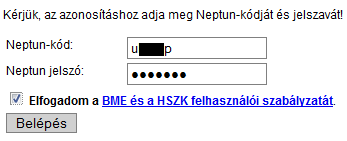
\includegraphics[width=0.50\textwidth]{figures/hszk_acc_admin_login.png}
\caption{Bejelentkezés a HSZK-s adminisztrációs oldalra \label{fig:hszk_acc_admin_login}}
\end{figure}

Sikeres bejelentkezés után keresd meg a \textit{HSZK Ural2 szerver használata} részt. Itt a második oszlopban találod a saját e-mailcímed felhasználói nevét (a kukac/@ előtti rész), amelyet jegyezz meg, ugyanis a következő részben ezzel fogsz tudni majd belépni a \href{https://webmail.hszk.bme.hu/}{https://webmail.hszk.bme.hu/} oldalon (\ref{fig:hszk_acc_admin_mailcim}. ábra). De előtte még beállítjuk a jelszavadat.

\begin{figure}[h!]
\centering
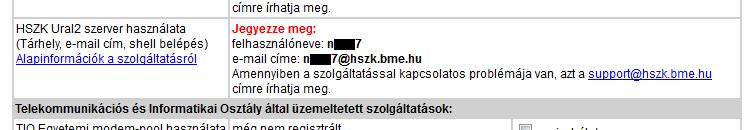
\includegraphics[width=0.80\textwidth]{figures/hszk_acc_admin_mailcim.png}
\caption{A HSZK-s emailcímed \label{fig:hszk_acc_admin_mailcim}}
\end{figure}

Az oldal alján keresd meg a jelszó beállításával kapcsolatos részt (\ref{fig:hszk_acc_admin_jelszo}. ábra). Itt adjál meg egy tetszőleges, a kívánt szabályoknak megfelelő jelszót, kattints a \textit{Fenti módosítások érvényesítése}, majd a \textit{Kilépés} gombra. A változások érvénybe lépéséhez kell egy kis idő. 

\begin{figure}[h!]
\centering
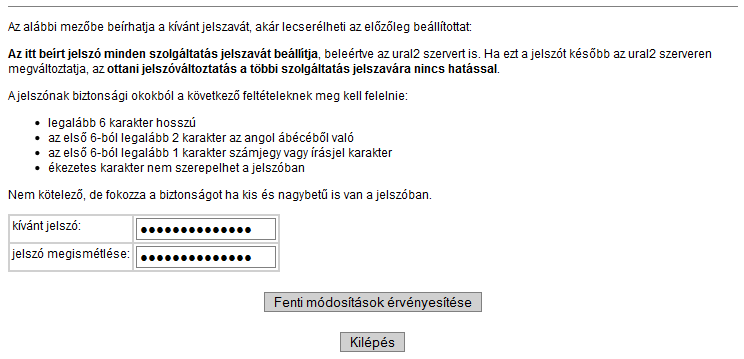
\includegraphics[width=0.80\textwidth]{figures/hszk_acc_admin_jelszo.png}
\caption{Jelszó beállítása \label{fig:hszk_acc_admin_jelszo}}
\end{figure}

\subsection{Belépés a HSZK-s webes postafiókba}

Amennyiben sikerült beállítanod az új jelszavadat, akkor látogasd meg a \href{https://webmail.hszk.bme.hu/}{https://webmail.hszk.bme.hu/} oldalt. Itt a felhasználói névnek írd be az előbb említett \textit{"betűbetűszám"} alakú felhasználói nevedet és az újonnan beállított jelszavadat. Ha elsőre nem sikerülne, ne ijedj meg, lehet, hogy még nem sikerült az új jelszónak bekerülni a rendszerbe. Ilyenkor várj néhány percet. Ha viszont sokáig hibaüzenetet kapsz, akkor érdemes lehet vissza menni a HSZK-s admin felületre (\href{https://accadmin.hszk.bme.hu/}{https://accadmin.hszk.bme.hu/}) és újra megpróbálni megadni egy jelszót, hátha elírtad.

Ha sikerült belépned, akkor egyelőre hagyjuk ezt az oldalt, és elkezdjük a regisztráció folyamatát.

\section{Regisztráció a jelentkező felület oldalán}

Látogasd meg a \href{https://jelentkezes.tnt.bme.hu}{https://jelentkezes.tnt.bme.hu} oldalt, és itt kattints a \textit{Regisztráció} gombra. Ezután add meg a \textbf{neptunkódodat} és egy tetszőleges jelszót (ennek nem kell megegyeznie a neptunban használt jelszavaddal), majd kattints a \textit{Regisztrálok} gombra.

Ezután a rendszer néhány perc múlva egy e-mailt küld a HSZK-s címedre. Látogasd meg megint a \href{https://webmail.hszk.bme.hu/}{https://webmail.hszk.bme.hu/} oldalt, lépj be és nyisd meg az e-mailt. Ebben találsz egy linket, amelyre ha rákattintasz aktiválod a fiókodat. Ezután a \href{https://jelentkezes.tnt.bme.hu}{https://jelentkezes.tnt.bme.hu} oldal \textit{Bejelentkezés} gombjára kattintva, és a szükséges bejelentkezési adatokat megadva már be tudsz lépni a rendszerbe.

\section{A jelentkezés felület használata}

Ezt a részt szerintem nem kell nagyon részletezni. Miután sikeresen beléptél, a rendszer kéri a neved, majd a következő oldalon a \textit{Tárgy, kurzus felvétele/módosítása} linkre kattintva megjelenik egy táblázat időpontokkal és sportágakkal. Nefelejtsd el megadni az oldal tetején, hogy a neptunban melyik tárgyat vetted fel, majd a számodra megfelelő kurzus kiválasztása után kattints az oldal alján a \textit{Mentés} gombra. Ezután a \textit{Profil} oldalon lévő táblázatban meg kell jelennie a felvett tárgynak, és kurzusnak.

Ezzel be is fejeztük a munkát, nyugodtan kijelentkezhetsz. 

\end{document}